%-------------------------------------------
\begin{frame}{Literate programming}

Literate programming

\end{frame}

%------------------------------------------------------------
\subsection{Introduction}

%-------------------------------------------
\begin{frame}{Introduction}

What is literate programming ?

\begin{definition}
"Literate programming is a \textbf{programming paradigm} introduced by Donald Knuth in which a computer program is given an explanation of its logic in a \textbf{natural language}, such as English, \textbf{interspersed with snippets of macros and traditional source code}, from which compilable source code can be generated."
\end{definition}


Wikipedia, 18/08/2020 (https://en.wikipedia.org/wiki/Literate\_programming\#Workflow)
\end{frame}

%-------------------------------------------
\begin{frame}{Introduction}

What does it look like ?

\centering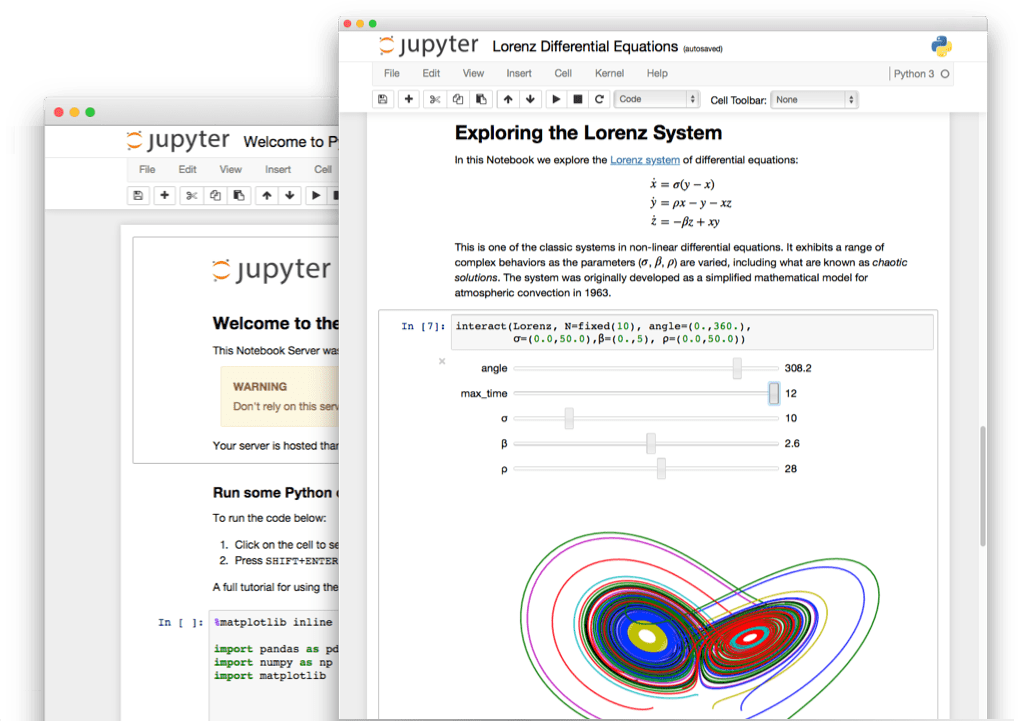
\includegraphics[width=10cm]{07_notebook/images/literate_programming.png}

\end{frame}

%-------------------------------------------
\begin{frame}{Introduction}
\begin{columns}

\column{0.5\textwidth}
\centering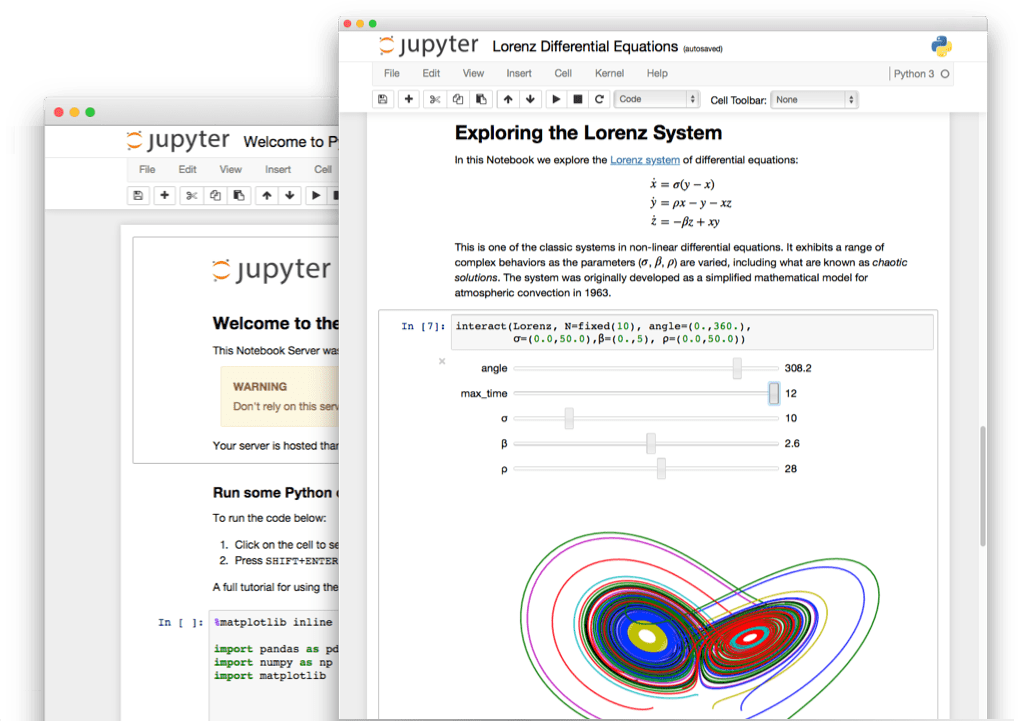
\includegraphics[width=6cm]{07_notebook/images/literate_programming.png}

\column{0.5\textwidth}
Interactive programming interface allowing to combine both natural and computer languages.
\newline
\newline
In one file:
\begin{itemize}
  \item Explanations
  \item Code
  \item Results
  \item Graphs and plots
\end{itemize}

\end{columns}
\end{frame}

%-------------------------------------------
\begin{frame}{Introduction}

Why using literate programming frameworks ?\newline
\newline
Use cases:
\begin{itemize}
  \item Day to day analyses
  \item Analysis reports
  \item Writing scientific articles
\end{itemize}

\end{frame}

%-------------------------------------------
\begin{frame}{Example of an article entirely written using a notebook}
\begin{columns}

\column{0.3\textwidth}
File (on a repository)\newline
\newline
\centering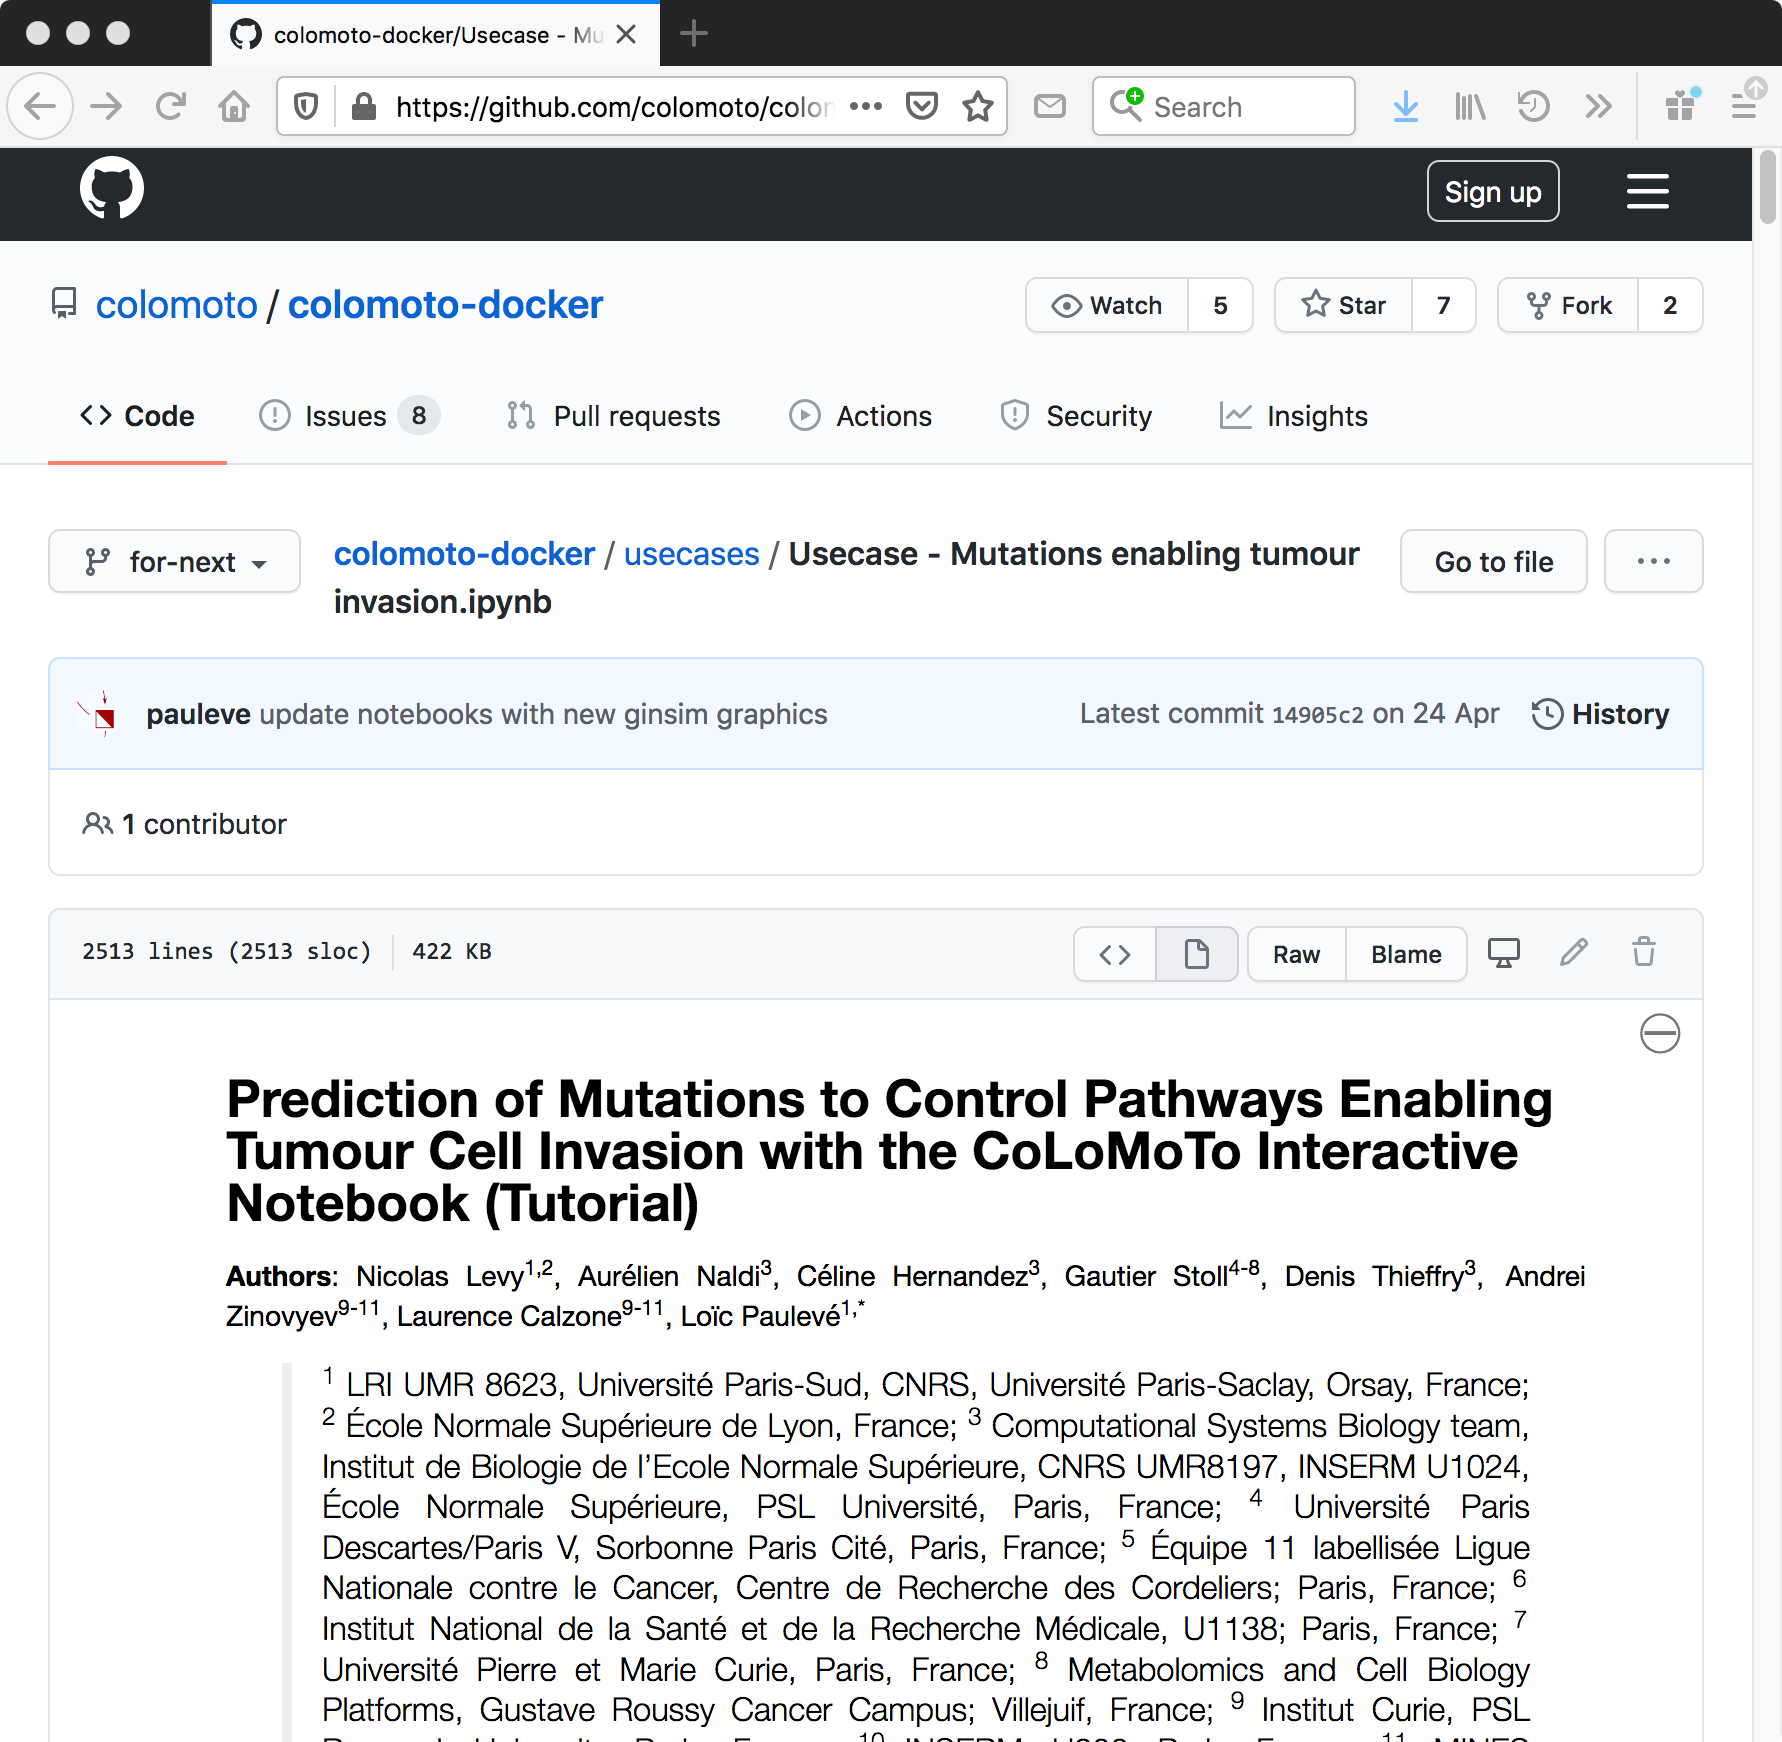
\includegraphics[width=3cm]{07_notebook/images/article_github.png}

\column{0.3\textwidth}
Published article\newline
\newline
\centering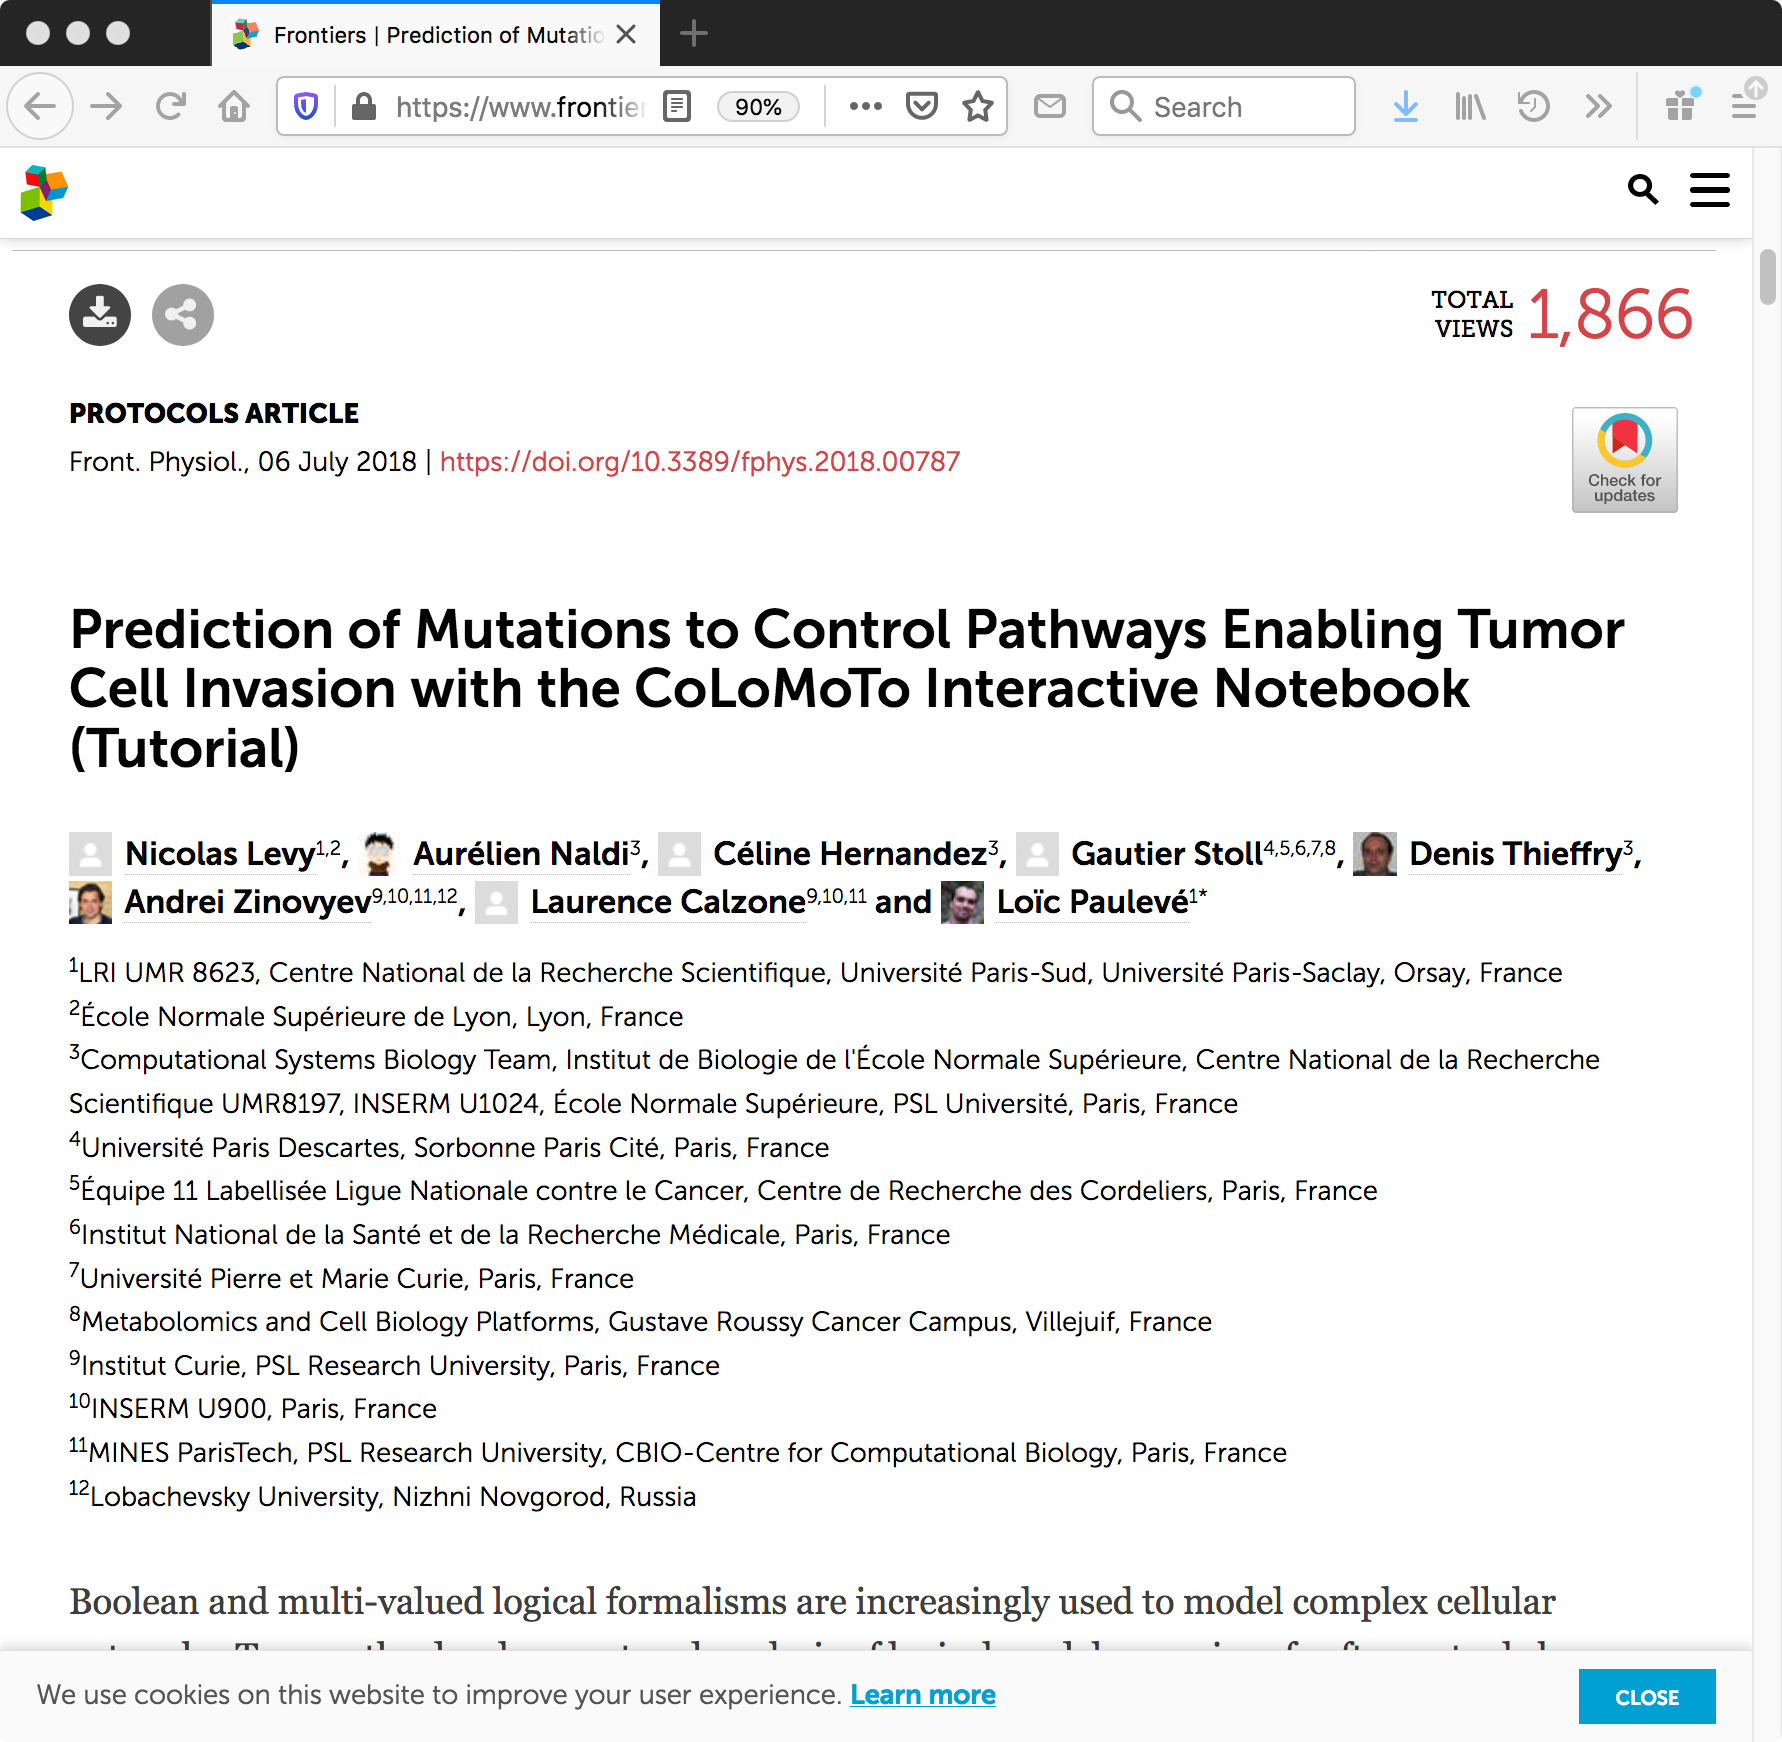
\includegraphics[width=3cm]{07_notebook/images/article_frontiers.png}
%http://dx.doi.org/10.3389/fphys.2018.00787

\column{0.3\textwidth}
Executable file\newline
\newline
\centering
\includegraphics[width=3cm]{07_notebook/images/article_nbviewer.png}
%%https://nbviewer.jupyter.org/gist/pauleve/a86717b0ae8750440dd589f778db428f/Usecase%20-%20Mutations%20enabling%20tumour%20invasion.ipynb

\end{columns}
%\centering https://colomoto.github.io/colomoto-docker/

\end{frame}

%-------------------------------------------
%\begin{frame}{Literate programming}
%
%Available frameworks:
%\begin{itemize}
%  \item Rmarkdown / RStudio
%  \item Jupyter (ex-iPython Notebook)
%\end{itemize}
%\newline
%\newline
%Available for many languages (R, Python...)
%\end{frame}

%-------------------------------------------
\begin{frame}{Literate programming}

This session :
\begin{itemize}
  \item Markdown
  \item Rmarkdown and RStudio
  \item Jupyter
\end{itemize}

\end{frame}

%------------------------------------------------------------
\subsection{Markdown}

%-------------------------------------------
\begin{frame}{Markup and markdown}

\begin{definition}
A markup language uses tags to define elements within a document.
\end{definition}
%\newline
%\newline
\vfill
Three different types and usage :
\begin{itemize}
  \item Presentational (used by traditional word-processing systems)
  \begin{itemize}
      \item Markup is invisible
  \end{itemize}
  \item Procedural, provides instructions to process the text (e.g.\ TeX, PostScript)
  \begin{itemize}
      \item Markup is visible and can be directly manipulated by the author.
  \end{itemize}
  \item Descriptive, to label documents parts (e.g.\ LaTeX, HTML, XML...)
  \begin{itemize}
      \item Emphasizes the document structure.
  \end{itemize}
\end{itemize}

\end{frame}

%-------------------------------------------
\begin{frame}{Markdown language}

Markdown is a Lightweight markup language.

Designed to be :
\begin{itemize}
    \item easy to \textbf{write} using any generic text editor (plain-text-formatting syntax)
    \item easy to \textbf{read} in its raw form
\end{itemize}

\end{frame}

%-------------------------------------------
\begin{frame}{Markdown language}

You've probably see it already on GitHub (README), Wikipedia... 

\centering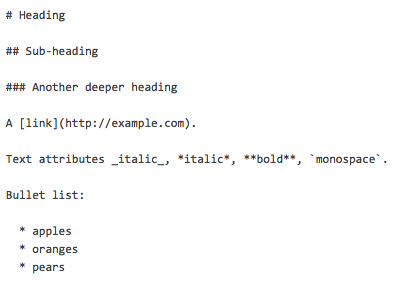
\includegraphics[width=8cm]{07_notebook/images/markdown.png}

Github guides : https://guides.github.com/features/mastering-markdown/
\end{frame}


%-------------------------------------------
\begin{frame}{Markdown language}

Une page de wiki est disponible sur FAIR\_bioinfo

https://github.com/thomasdenecker/FAIR\_Bioinfo/wiki/Markdown

\centering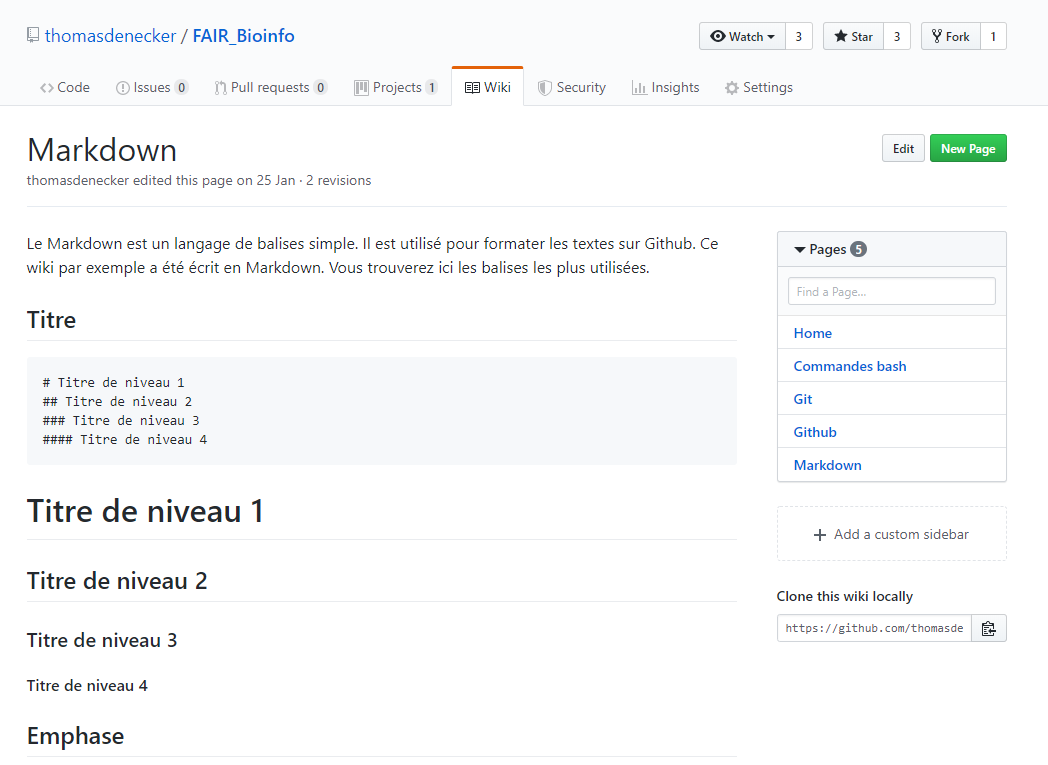
\includegraphics[width=8cm]{07_notebook/images/markdown_github_FAIR_bioinfo.png}

\end{frame}

